\documentclass{article}[18pt]
\usepackage{../../../../../format}
\lhead{Computational Thinking - ECC}
\usepackage{mathtools}


\begin{document}
\begin{center}
\underline{\huge ECC Lecture 1}
\end{center}
\section{Error control}
\subsection{Why error control?}
Messages are subject to errors when transmitted through a channel: spacial (data transmission) or temporal (storage)
\begin{center}
	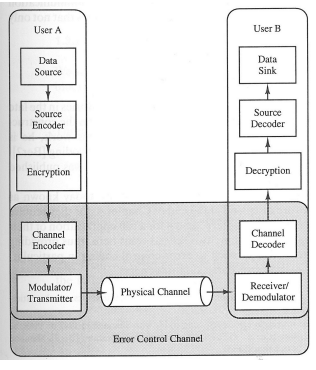
\includegraphics[scale=0.7]{ecc1}
\end{center}
\subsection{The tenets of error control}
Advantage of digital data v analog: we can perform error correction\\
\\
Main assumption:
\begin{itemize}
	\item Simplify the channel
	\item Suppose errors occur infrequently
\end{itemize}
Main idea: add redundancy to the data
\subsection{The codebook idea}
Everyday language uses a form of error control:\\
If you can't hear your friend in a crowded room, what do you do?\\
\\
Basic error control code: repetition\\
\\
The language itself is an error correcting code:\\
"I am going to the con\textbf{k}ert tonight"\\
Easy to detect and correct the error:\\
"I am going to the concert tonight"\\
\\
Some sequences of letters are correct, others are incorrect\\
The correct ones form a \textbf{code}
\section{Basic examples}
\subsection{Basic error detection}
\textbf{Parity-check code}: add one more bit to the sequence of bits so that the overall number of 1's is even\\
\\
Codebook: all sequences of a given length with an even number of bits equal to one\\
E.g. $1100011\xrightarrow{\text{encoding}}1100011\mathbf{0}$\\
\\
Used in first version of ASCII (7 bits for the symbol +1 parity check bit)
\subsection{Parity check code}
Can \textbf{detect one error} buy simply checking the number of ones
$$1100011\xrightarrow{\text{encoding}}11000110\xrightarrow{\text{channel}}110\textbf{1}0110$$
Cannot detect two errors
$$1100011\xrightarrow{\text{encoding}}11000110\xrightarrow{\text{channel}}110\textbf{11}110$$
Cannot correct any error: e.g. if we receive 11010110, what happened?
$$1100011\xrightarrow{\text{encoding}}11000110\xrightarrow{\text{channel}}110\textbf{1}0110 \quad or$$
$$1100011\xrightarrow{\text{encoding}}11000110\xrightarrow{\text{channel}}1101011\mathbf{0}$$
\subsection{Basic error correction}
\textbf{Repetition code:} send the same but multiple times
$$0\rightarrow 000$$
$$1\rightarrow 111$$
Codebook $\{000,111\}$\\
\\
Can \textbf{correct one error} e.g.
$$0\xrightarrow{\text{encoder}}000\xrightarrow{\text{channel}}0\mathbf{1}0\xrightarrow{\text{decoder}}0$$
$$1\xrightarrow{\text{encoder}}111\xrightarrow{\text{channel}}11\mathbf{0}\xrightarrow{\text{decoder}}1$$
Can detect two errors e.g. $0\rightarrow 00 \rightarrow \mathbf{11}0$\\
Very low rate 1/3, so we need more rate efficient techniques\\
\\
For n bits:
\begin{itemize}
	\item We can detect n-1 errors
	\item We can correct $\lfloor \frac{n-1}{2}\rfloor$ errors
\end{itemize}
$$t<m-t$$
$$2t<m$$
$$2t\leqslant m-1$$
As t is an integer
$$t\leqslant\Bigg\lfloor \frac{m-1}{2}\Bigg\rfloor$$
\subsection{Objectives}
We want to design a "good" error correcting code, i.e.
\begin{enumerate}
	\item Detects and corrects many errors
	\item High rate
	\item Easy to encode and decode
\end{enumerate}
The first two are conflicting: compromise depending on the channel quality
\section{Minimum distance}
\subsection{Hamming distance}
The \textbf{Hamming distance} between two sequences is the number of times they disagree. E.g. $d_H(100,101)=1$\\
It is a metric
\begin{enumerate}
	\item $d_H(x,y)\geqslant 0$
	\item $d_H(x,y)=d_H(y,x)$
	\item $d_H(x,y)=0$ iff $x=y$
	\item $d_H(x,y)\leqslant d_H(x,z)+d_H(z,y)$ (triangular inequality)
\end{enumerate}
In other words, it has a geometric meaning\\
\\
The Hamming weight of a sequence is simply the number of 1s in it
$$w_H(x)=d_H(x,0,...,0)$$
\subsection{Hamming distance and error correction}
\textbf{Decoding}: if it receives the sequence v, the decoder returns the unique nearest (in terms of Hamming distance) codeword to v if it exists.\\
\\
If the codeword is not unique we need a sufficient condition to make sure the decoding is non-ambiguous 
\subsection{Minimum distance}
\textbf{Definition}: $d_{min}(C)$ is the minimum distance between two distinct codewords in C\\
\textbf{Theorem}: a code can correct t errors iff it has minimum distance $d_{min}\geqslant 2t+1$
\end{document}